\documentclass{beamer}
\usetheme{Antibes}
\usepackage{xcolor, colortbl}
\usepackage{algorithm}
\usepackage{algpseudocode}
\usepackage{textcomp}
\usepackage{listings}
\usepackage{hyperref}
\usepackage{alltt}
\usepackage{tikz}
\usepackage{framed}
\usepackage{marvosym}
\usepackage{wasysym}
\usepackage{marvosym}
\usepackage{crayola}
\usepackage{mathpartir}
\usepackage{tabularx}
\usepackage[belowskip=-15pt,aboveskip=0pt]{caption}
\usepackage[skins]{tcolorbox}
\usepackage{multicol}
\usetikzlibrary{positioning,shapes,arrows, backgrounds, fit, shadows, automata}
\usetikzlibrary{decorations.markings, calc}
%\usepackage{wasysym}
%\usepackage{marvosym}
\setbeamertemplate{footline}[frame number]
%\usecolortheme{fly}
\usefonttheme{serif}

\title[Sujit]{Lexical Analysis \\
Programming Languages}
\author{Sujit Kumar Chakrabarti}
\institute{IIITB}
\date{}


\definecolor{lightblue}{rgb}{0.8,0.93,1.0} % color values Red, Green, Blue
\definecolor{darkblue}{rgb}{0.4,0.3,1.0} % color values Red, Green, Blue
\definecolor{Blue}{rgb}{0,0,1.0} % color values Red, Green, Blue
\definecolor{darkgreen}{rgb}{0,0.7,0.2} % color values Red, Green, Blue
\definecolor{Red}{rgb}{1,0,0} % color values Red, Green, Blue
\definecolor{Pink}{rgb}{0.7,0,0.2}
\definecolor{links}{HTML}{2A1B81}
\definecolor{mydarkgreen}{HTML}{126215}
\newcommand{\highlight}[1]{{\color{Red}(#1)}}

\newcommand{\myheader}[1]{
	{\color{darkblue}
		\begin{Large}
			\begin{center}
				{#1}
			\end{center}
		\end{Large}
	}
}
\newcommand{\myminorheader}[1]{
	{\color{BrickRed}
		\begin{Large}
			{\fontfamily{\sfdefault}\selectfont\textbf{#1}}
		\end{Large}
	}
}

%\tikzstyle{input} = [coordinate]
%\tikzstyle{output} = [coordinate]


\tikzstyle{bb}=[%
      rectangle, draw=black, thick, fill=OliveGreen!30, drop shadow, align=center,
      text ragged, minimum height=2em, minimum width=2em, inner sep=6pt
]

\tikzstyle{inv}=[%
      rectangle, draw=none,  align=center,
      text ragged, minimum height=2em, minimum width=2em, align=center, inner sep=6pt
]

\tikzstyle{db}=[%
      ellipse, draw=black, thick, fill=pink, drop shadow, align=center,
      text ragged, minimum height=2em, inner sep=6pt
]

\tikzstyle{jn}=[%
      inner sep=0cm, outer sep=0cm
]

\tikzstyle{io}=[%
      trapezium, trapezium left angle=60, trapezium right angle=120, draw=black, thick, fill=brown, drop shadow,
      text ragged, minimum height=2em, minimum width=2em, inner sep=6pt, align=center
]

\tikzstyle{glio}=[%
      trapezium, trapezium left angle=60, trapezium right angle=120, draw=red, line width = 1mm, fill=brown, drop shadow,
      text ragged, minimum height=2em, minimum width=2em, inner sep=6pt
]
\tikzstyle{gl}=[%
      rectangle, draw=red, line width = 1mm, fill=lightblue, drop shadow,
      text ragged, minimum height=2em, minimum width=2em, inner sep=6pt
]

\tikzstyle{en}=[%
      rectangle, draw=black, thick, fill=none,
      text ragged, minimum height=2em, minimum width=2em, inner sep=6pt
]

\tikzstyle{sh}=[%
      rectangle, draw=gray, thick, fill=none, color = gray,
      text ragged, minimum height=2em, minimum width=2em, inner sep=6pt
]


\lstdefinestyle{javacode}{
	language = Java,
	basicstyle = \ttfamily\scriptsize,
	stringstyle = \ttfamily,
	keywordstyle=\color{Blue}\bfseries,
	identifierstyle=\color{Pink},
	commentstyle=\color{darkgreen},
	frame=single,
	frameround=tttt,
%	numbers=left
	showstringspaces=false
}

\lstdefinestyle{camlcode}{
	language = Caml,
	basicstyle = \scriptsize\ttfamily,
	stringstyle = \color{red}\ttfamily,
	keywordstyle=\color{Blue}\bfseries,
	identifierstyle=\ttfamily,
	frame=single,
	frameround=tttt,
	numbers=none,
	showstringspaces=false,
	escapeinside={(*@}{@*)}
}

\lstdefinestyle{outputcode}{
	language = bash,
	backgroundcolor = \color{black},
	basicstyle = \tiny\ttfamily\color{white},
	stringstyle = \color{red}\ttfamily,
	keywordstyle=\color{white}\bfseries,
	identifierstyle=\ttfamily,
	frameround=tttt,
	numbers=none,
	showstringspaces=false,
	escapeinside={(*@}{@*)}
}

\newtcolorbox{myframe}[2][]{%
  enhanced,colback=white,colframe=black,coltitle=black,
  sharp corners,boxrule=0.4pt,
  fonttitle=\itshape,
  attach boxed title to top left={yshift=-0.3\baselineskip-0.4pt,xshift=2mm},
  boxed title style={tile,size=minimal,left=0.5mm,right=0.5mm,
    colback=white,before upper=\strut},
  title=#2,#1
}

\begin{document}
\maketitle

\section{Manual Implementation of Lexical Analysis}
% frame begin %%%%%%%%%%%%%%%%%%%%%%%%
\begin{frame}[fragile]{Automatic Generation of Lexical Analysis}
{Introduction}

\begin{enumerate}
\item Belongs to the Lex family of tools
\item First created in AT\&T Bell Labs in 1975
\item Several implementations

\begin{center}
\begin{scriptsize}
\begin{tabular}{| l | l |}
\hline
Programming Language & Implementation \\
\hline
C & Lex \\
C++ & flex \\
Java & JLex \\
OCaml & Ocamllex \\
... & ... \\
\hline
\end{tabular}
\end{scriptsize}
\end{center}
\end{enumerate}

\end{frame}
% frame end %%%%%%%%%%%%%%%%%%%%%%%%

% frame begin %%%%%%%%%%%%%%%%%%%%%%%%
\begin{frame}[fragile]{Automatic Generation of Lexical Analysis}
{Schematic}

\begin{center}
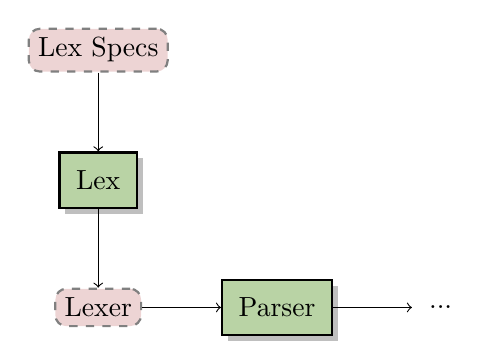
\begin{tikzpicture}
\node[draw=Gray, dashed, thick, fill=Brown!20, rounded corners] (spec) {Lex Specs};
\node[bb, below=of spec](lex) {Lex};
\node[draw=Gray, dashed, thick, fill=Brown!20, rounded corners, below=of lex] (lexer) {Lexer};

\draw[->] (spec) to (lex);
\draw[->] (lex) to (lexer);
\pause
\node[bb, right=of lexer] (parser) {Parser};
\node[inv, right=of parser] (others) {...};

\draw[->] (lexer) to (parser);
\draw[->] (parser) to (others);

\end{tikzpicture}
\end{center}
\end{frame}
% frame end %%%%%%%%%%%%%%%%%%%%%%%%

% frame begin %%%%%%%%%%%%%%%%%%%%%%%%
\begin{frame}[fragile]{Automatic Generation of Lexical Analysis}
{Specification File}

\begin{lstlisting}[style=camlcode]
(* PART ONE *)
OCaml code to be pasted verbatim.

(* PART TWO *)
Lexical Specification

(* PART THREE *)
Additional OCaml code.

\end{lstlisting}
\end{frame}
% frame end %%%%%%%%%%%%%%%%%%%%%%%%

% frame begin %%%%%%%%%%%%%%%%%%%%%%%%
\begin{frame}[fragile]{Automatic Generation of Lexical Analysis}
{Demo}

\begin{scriptsize}

\begin{enumerate}
\item Example
\item MLL file structure
\item Last token recognised
\item String literal
\end{enumerate}
\end{scriptsize}
\end{frame}
% frame end %%%%%%%%%%%%%%%%%%%%%%%%

\end{document}
